\documentclass{SciPress_2015}

%!!!!!!!!!!!!!!!!!!!!!!!!!!!!!!!!!!!!!!!!!!!!!!!!!!!!!!!!!!!!!!!!!!!!!
%---PLEASE USE XeLaTeX PACKAGE TO COMPILE THE TeX  FILE
%!!!!!!!!!!!!!!!!!!!!!!!!!!!!!!!!!!!!!!!!!!!!!!!!!!!!!!!!!!!!!!!!!!!!!

%--------------------------------------------- Basic packages (could be expanded by author)%
\usepackage{graphicx}
\usepackage{tabularx}
\usepackage{array}
\usepackage{makecell}
\usepackage{float}
\usepackage{amsmath}
\usepackage{amssymb}
\usepackage{exscale}
\usepackage{nameref}
\usepackage{hyperref}
\usepackage{enumitem}
\usepackage{times}
%\usepackage{xparse}
\usepackage{fontspec}
\usepackage{subfigure}
\usepackage[usenames]{color}

\newcolumntype{L}{>{\begin{math}}l<{\end{math}}}%
\newcolumntype{C}{>{\begin{math}}c<{\end{math}}}%
\newcolumntype{R}{>{\begin{math}}r<{\end{math}}}%

\setlength{\skip\footins}{1.4pc plus 5pt minus 2pt}

%\usepackage{fontspec-patches}	
% <-- DO NOT REMOVE this package,
% because the fonts (Times New Roman and Arial) will not be used in the document.
% If you don`t have this package, you can get it from the Internet or you can get this
% package from the archive The_Fontspec_package.zip which you downloaded with
% this current file.
%---------------------------------------------If you need include the .eps files, please uncomment the package bellow.%
%\usepackage{epsfig}
%--------------------------------------------- Override fonts to Times New Roman and Arial%
\renewcommand{\large}{\fontsize{14}{18pt}\selectfont}
\renewcommand{\small}{\fontsize{11}{13.6pt}\selectfont}
\setmainfont{Times New Roman}
\setsansfont{Arial}
%--------------------------------------------- New commands for quick editing of the document%
\newcommand{\titleformat}{\sffamily\bfseries \large}						%	<--- Doc. title
\newcommand{\authorformat}{\sffamily \large}							%	<--- Authors
\newcommand{\keywordsformat}{\noindent \small \sffamily}				%	<--- Kyewords
\newcommand{\abstractformat}{\noindent \textbf}						%	<--- Abstract
\newcommand{\contentformat}{\rmfamily \normalsize \vspace{18pt}}			%	<--- Main content
\newcommand{\email}{\sffamily \small \vspace{-8pt}}						%	<--- E-mail
\renewcommand{\subsection}[1]{\textit{\textbf{#1}}}

%--------------------------------------------- Make all internal and external links - black color%
\hypersetup{
    colorlinks,%
    citecolor=black,%
    filecolor=black,%
    linkcolor=black,%
    urlcolor=black
}
%--------------------------------------------- Set the basic parameters of the page. DO NOT CHANGE!%
\special{papersize=210mm,297mm}
\textheight=25.6cm
%--------------------------------------------- For the Publisher to Enter:

\begin{document}
\title{\titleformat Divisions by Two in Collatz Sequences:\\
	A Data Science Approach}

\author{\authorformat Christian Koch\inst{1}$^{,\rm{a{\rm{*}}}}$\textbf{,}
	Eldar Sultanow \inst{2}$^{,\rm{b}}$ and Sean Cox
\inst{3}$^{,\rm{c}}$}
\institute{\sffamily $^{\rm 1}$Technische Hochschule Nürnberg Georg Simon Ohm, Nuremberg, Germany\\
        \vspace{8pt} $^{\rm 2}$Capgemini, Nuremberg, Germany\\
        \vspace{8pt} $^{\rm 3}$RatPac-Dune Entertainment, Los Angeles, USA
}

\maketitle
\begin{center}
\vspace{2pt}\email{ $^{\rm a}$christian.koch@th-nuernberg.de,
	$^{\rm b}$eldar.sultanow@capgemini.com,
	$^{\rm c}$sean.cox@ratpacent.com}
\end{center}

\keywordsformat{{\textbf{Keywords:}Collatz Conjecture, Divisions by Two, Binary Representation, Data Science}}

\contentformat
\abstractformat{Abstract.}
The Collatz conjecture is an unsolved number theory problem. We approach the question by examining the divisions by two that are performed within Collatz sequences. Aside from classical mathematical methods, we use techniques of data science. Based on the analysis of 10,000 sequences we show that the number of divisions by two lies within clear boundaries. Building on the results, we develop and prove an equation to calculate the maximum possible number of divisions by two for any given Collatz sequence. Whenever this maximum is reached, a sequence leads to the result one, as conjectured by Lothar Collatz. Furthermore, we show how many divisions by two are required for a cycle of a specific length. The findings are valuable for further investigations and could form the basis for a comprehensive proof of the conjecture.

\section{Introduction}
\subsection{The Problem}
\par\noindent
The Collatz conjecture is a well-known number theory problem and is the subject of numerous publications.\footnote{An overview is provided by Lagarias \cite{Ref_Lagarias_2010}.} Therefore, our description of the topic will be brief. The mathematician Lothar Collatz introduced a function $g:\mathbb{N}\rightarrow\mathbb{N}$ as follows:

\begin{equation}
\label{eq:func_collatz}
g(x)=
\begin{cases}
3x+1	&	\text{if}\ x\equiv 1(\textrm{mod}\ 2)\\
x/2		&	\text{if}\ x\equiv 0(\textrm{mod}\ 2)
\end{cases}
\end{equation}

The conjecture, as treated in this paper, claims that the above function leads to the final result one for every natural starting number, when applied recursively. A series of numbers involved in this process is called a Collatz sequence. With an aim to contribute to a proof of the conjecture, this paper analyses a central aspect of the problem: the divisions by two.\footnote{Details on our scientific approach can be found in appendix "\nameref{appx:scientific_approach}".}

\vspace{1em}\noindent
\subsection{Determining Odd Numbers}
\par\noindent
Sultanow, Koch and Cox demonstrated that odd numbers of Collatz sequences can be calculated with the following recursive equation:\footnote{See Sultanow, Koch, and Cox \cite[p.~10]{Ref_Sultanow_Koch_Cox_2020}.}
\begin{equation}
\label{eq:reachability_3}
v_{n+1}=3^n\cdot v_1\cdot\prod_{i=1}^{n}\left(1+\frac{1}{3v_{i}}\right)\cdot\prod_{i=1}^{n}2^{-\alpha_i}
\end{equation}

The variable $v_1$ denotes the first odd number of the sequence, that is, the starting value. The variable $v_i$ symbolises the odd number that is the result of a particular iteration.\footnote{For $n=1$ this is the starting value $v_1$.} The exponent $n$ stands for the count of odd numbers that are processed by the algorithm. In the further course of this paper we will call the parameter $n$ the \textit{length} of a sequence. The exponent $\alpha_i$ finally represents the number of divisions by two that are performed in a specific iteration. Accordingly, the sum of $\alpha_i$ is the count of divisions by two leading from the starting value $v_1$ to the outcome $v_{n+1}$.\footnote{For a glossary of notations see section "\nameref{appx:glossary_of_notations}" in the appendix.} Let us consider the example $v_1=13$ and $n=2$. Applying equation~\ref{eq:reachability_3} yields:\footnote{The result of the first iteration $v_{1+1}$ equals five.}
\[
v_{2+1}=3^2\cdot 13\cdot\left(1+\frac{1}{3\cdot13}\right)\cdot\left(1+\frac{1}{3\cdot5}\right)\cdot2^{-7}=1
\]

\par\noindent
Starting with $v_1=33$ for $n=3$ we obtain the result:
\[
v_{3+1}=3^3\cdot 33\cdot\left(1+\frac{1}{3\cdot33}\right)\cdot\left(1+\frac{1}{3\cdot25}\right)\cdot\left(1+\frac{1}{3\cdot19}\right)\cdot2^{-5}=29
\]

Improving readability, we denote the factor $\left(1+\frac{1}{3\cdot v_i}\right)$ with the variable $\beta_i$. In addition, we generalise the formula by replacing the factor three with the variable $k$. This will be useful for further analysis and leads us to the following generalised version of equation~\ref{eq:reachability_3}:
\begin{flalign}
\label{eq:reachability_k}
v_{n+1}&=k^n\cdot v_1\cdot\prod_{i=1}^{n}\left(1+\frac{1}{kv_{i}}\right)\cdot\prod_{i=1}^{n}2^{-\alpha_i}\\
\notag
v_{n+1}&=k^n\cdot v_1\cdot\prod_{i=1}^{n}\beta_i\cdot\prod_{i=1}^{n}2^{-\alpha_i}
\end{flalign}

In order to correctly calculate odd numbers with formula~\ref{eq:reachability_k}, we must first define the halting conditions of the algorithm in the next section.

\vspace{1em}\noindent
\subsection{Halting Conditions}
\label{sec:halting_conditions}
\par\noindent
Being compliant with the Collatz conjecture, the algorithms~\ref{eq:reachability_3} and \ref{eq:reachability_k} halt if at least one of the following conditions is fulfilled:
\begin{equation}
\label{eq:halting_condition}
\begin{array}{ll}
\text{1.}&v_{n+1}=1\\[\medskipamount]
\text{2.}&v_{n+1}\in\{v_1,v_2,v_3,\ldots,v_n\}
\end{array}
\end{equation}

When the first condition applies, the Collatz conjecture is true for a specific sequence. If the second condition is fulfilled, the sequence has led to a cycle. For every starting value, except $v_1=1$, the Collatz conjecture is therefore falsified.\footnote{This statement refers to the Collatz conjecture in its original form $3v+1$.} Let us consider the example $k=3$, $v_1=13$, and $n=2$. Applying equation~\ref{eq:reachability_k} yields:
\[
v_{2+1}=3^2\cdot 13\cdot\left(1+\frac{1}{3\cdot13}\right)\cdot\left(1+\frac{1}{3\cdot5}\right)\cdot2^{-7}=1
\]

In the above example the algorithm halts after two iterations because the first condition is fulfilled. If we examine the case $v_1=1$, we realise that the algorithm finishes after the first iteration, since both halting conditions are true:
\[
v_{1+1}=v_1=3^1\cdot 1\cdot\left(1+\frac{1}{3\cdot1}\right)\cdot2^{-2}=1
\]

The sequence stops in the example above due to the result being one. Apart from that, the sequence has led to a cycle.

\section{Boundaries of \boldmath$\alpha_i$}
We know that in every iteration of the equations~\ref{eq:reachability_3} and \ref{eq:reachability_k} at least one division by two is performed. This follows from the constraints of the Collatz problem. Consequently, we can define the minimum of $\alpha_i$ with the following condition:
\[
1\le\alpha_i
\]

The maximum can be specified in a similarly easy way. According to the halting conditions, defined in the previous section, a Collatz sequence finishes when $v_{n+1}=1$. The maximum of $\alpha_i$, hereinafter called $\hat\alpha_i$, can hence be defined as:
\begin{equation}
\label{eq:alpha_max}
\begin{array}{l}
2^{\hat\alpha_i}=k\cdot v_i+1\\[\medskipamount]
\hat\alpha_i=\log_2k+\log_2v_i+\log_2\beta_i
\end{array}
\end{equation}

The formula above builds on the fact that the expression $2^{\hat\alpha_i}$ must equal the next even number $k\cdot v_i+1$ in order to lead to $v_{n+1}=1$. Being greater, the result $v_{n+1}$ would be less than one. The second step inverses the exponentiation of $\hat\alpha_i$ by taking the binary logarithm. Appropriately, we replace the operation \textit{plus one} by $\beta_i$. For a better understanding of the above term, let us consider the example $k=3$ and $v_1=5$. In this case equation~\ref{eq:alpha_max} results in:
\[
\alpha_1=\hat\alpha_1=4=\log_23+\log_25+\log_2\left(1+\frac{1}{3\cdot5}\right)
\]

Whenever a sequence reaches the maximum $\hat\alpha_i$, it finishes with one, thus verifying the Collatz conjecture. If we could prove that every odd number finally leads to this maximum for $k=3$, the Collatz problem would be solved. Summarising, we can define the following boundaries for $\alpha_i$:
\begin{equation}
\label{eq:boundary_alpha_i}
1\le\alpha_i\le\log_2k+\log_2v_i+\log_2\beta_i
\end{equation}

Before we continue, we validate theorem~\ref{eq:boundary_alpha_i} empirically. We will do so at various points in this paper to avoid obvious errors in our mathematical reasoning. The basis for the validation is a sample of $10,000$ Collatz sequences. The data set comprises information about sequences for the odd starting numbers $v_1\in\{1,3,5,\ldots,3999\}$ and $k\in\{1,3,5,7,9\}$. Since we do not know that all generated sequences halt, we limited the number of iterations per sequence to $n=100$. For further details on the data set, see section "\nameref{appx:data_set}" in the appendix.

Unsurprisingly, we found that all values of $\alpha_i$ in the sample are compliant with theorem~\ref{eq:boundary_alpha_i}.\footnote{Source: Own empirical analysis, see appendix "\nameref{appx:data_set}" for details.} In the next section we move on to more sophisticated considerations and study the properties of $\prod_{1}^{n}2^{\alpha_i}$.

\section{Analysing \boldmath$\alpha$}
\label{sec:analysing_alpha}
\subsection{Boundaries of \boldmath$\alpha$}
\par\noindent
In equations~\ref{eq:reachability_3} and \ref{eq:reachability_k}, the expression $\prod_{i=1}^{n}2^{\alpha_i}$ represents the divisions by two performed by the algorithms. The number of divisions by two can be determined with the following formula and will be symbolised by $\alpha$:

\[
\alpha=\sum_{i=1}^{n}{\alpha_i}
\]

\newpage
\par\noindent
Based on theorem~\ref{eq:boundary_alpha_i} we can define the minimum of α as follows:
\[
n\le \alpha
\]
Since we carry out at least one division by two in every iteration of formulas~\ref{eq:reachability_3} and \ref{eq:reachability_k}, the minimum of $\alpha$ equals the sequence's length. The maximum value is harder to determine. In the first step we derive it empirically from the data set mentioned in the previous section. Based on the observed data we formulate the hypothesis that the maximum of $\alpha$ can be calculated with the following equation:
\begin{equation}
\label{eq:max_alpha}
\begin{array}{l}
\hat\alpha=\lfloor n\cdot\log_2k+\log_2v_1\rfloor+1\\[\medskipamount]
\alpha\le\hat\alpha
\end{array}
\end{equation}

The hypothesis holds for all Collatz sequences in the empirical data set.\footnote{Source: Own empirical analysis, see appendix "\nameref{appx:data_set}" for details.} If a Collatz sequence reaches the above stated maximum, it finishes with one, as conjectured by Lothar Collatz.\footnote{The parameter $n$, representing the length of a sequence, cannot be predicted for a specific $k$ and $v_1$ with the formula.} Let us, for example, consider the case where $v_1=13$, $n=2$ and $k=3$. Applying theorem~\ref{eq:max_alpha} and formula~\ref{eq:reachability_k} leads to:
\[
\begin{array}{l}
\hat\alpha=\lfloor 2\cdot\log_23+\log_213\rfloor+1=7\\[\medskipamount]
v_{2+1}=3^2\cdot 13\cdot\left(1+\frac{1}{3\cdot13}\right)\cdot\left(1+\frac{1}{3\cdot5}\right)\cdot2^{-7}=1
\end{array}
\]

\par\noindent
The empirical validation supports our hypothesis, but does not prove it for all Collatz sequences. Throughout the next sections we will formulate a comprehensive proof of theorem~\ref{eq:max_alpha} step by step.

\vspace{1em}\noindent
\subsection{Proving \boldmath$\hat\alpha$ for \boldmath$k=1$}
\par\noindent
First, we examine the case $k=1$, where theorem~\ref{eq:max_alpha} can be simplified as follows:
\begin{equation}
\label{eq:max_alpha_1}
\hat\alpha=\lfloor n\cdot\log_21+\log_2v_1\rfloor+1=\lfloor\log_2v_1\rfloor+1
\end{equation}

\par\noindent
In order to prove theorem~\ref{eq:max_alpha}, we have to demonstrate that the number of divisions by two, $\alpha$, is less than or equal to the maximum $\hat\alpha$. This can be achieved by analysing the binary representation of Collatz numbers.\footnote{To avoid confusion between decimal and binary numbers, we will label binary numbers with a subscripted $2$.} Let us consider the case $v_1=25$ and $k=1$ in the decimal system. Applying equation~\ref{eq:reachability_k} leads to the sequence shown in the following table.

\begin{table}[H]
	\centering
	\begin{tabular}{|L|L|R|R|R|R|R|R|R|}
		\hline
		\thead{\boldmath$n$} &
		\thead{\textbf{variable}} &
		\thead{\textbf{decimal}} &
		\thead{\boldsymbol{\log2}} &
		\thead{\textbf{binary}} &
		\thead{\textbf{binary length}} &
		\thead{\boldsymbol{\alpha_i}} &
		\thead{\boldsymbol{\alpha}} &
		\thead{\textbf{operation}} \\
		\hline
		\multirowcell{2}1 & v_1 & 25 & 4.64 & 11001_2 & 5 & & & +1
		\\ \cline{2-9}
		& v_1+1 & 26 & 4.70 & 11010_2 & 5 & 1 & 1 & \cdot2^{-1}
		\\ \hline
		\multirowcell{2}2 & v_2 & 13 & 3.70 & 1101_2 & 4 & & & +1
		\\ \cline{2-9}
		& v_2+1 & 14 & 3.81 & 1110_2 & 4 & 1 & 2 & \cdot2^{-1}
		\\ \hline
		\multirowcell{2}3 & v_3 & 7 & 2.81 & 111_2 & 3 & & & +1
		\\ \cline{2-9}
		& v_3+1 & 8 & 3.00 & 1000_2 & 4 & 3 & 5 & \cdot2^{-3}
		\\ \hline
		4 & v_4 & 1 & 1.00 & 1_2 & 1 & & &
		\\ \hline
	\end{tabular}
	\caption{Binary representation of a Collatz sequence for $k=1$}
	\label{table:k_1}
\end{table}

\par\noindent
The sequence presented in table~\ref{table:k_1} starts with the decimal number $v_1=25$ at $n=1$. Subsequently it comprises the odd numbers $v_2=13$, $v_3=7$ and finally $v_4=1$. In the binary system the sequence starts accordingly with $v_1=11001_2$. The binary length of the starting number $len(v_1)$ equals five.\footnote{With binary length we mean the count of digits of a binary number.} This observation is crucial for our proof. For clarification, it is important to note that the length of a binary number can be calculated with the following equation:\footnote{See Sedgewick and Wayne \cite[p.~185]{Ref_Sedgewick_Wayne_2011}.}
\begin{equation}
\label{eq:binary_length}
len(v_i)=\lfloor\log_2v_i\rfloor+1
\end{equation}

For example, consider the case $v_i=13$ in decimal, rendered in binary that means $v_i=1101_2$. Here, equation~\ref{eq:binary_length} leads to the following result:
\[
len(13)=len(1101_2)=\lfloor\log_213\rfloor+1=4
\]

The comparison of equation~\ref{eq:binary_length} with formula~\ref{eq:max_alpha_1} makes it clear that they are identical. This raises the question why the maximum number of divisions by two of a Collatz sequence corresponds to the binary length of $v_1$.\footnote{The statement is only true for $k=1$.} To answer this, we take a closer look at the mechanics of a Collatz sequence in the binary system.

\par\medskip
We start with $v_1=11001_2$ in the above example. Adding one, we obtain the even number $v_1+1=11010_2$. The binary length of $v_1$ equals the binary length of $v_1+1$, which is five. Due to the trailing zero we immediately realise that $v_1+1$ is even. A division by two can be performed in the binary system by deleting the trailing zero. The result is $v_2=1101_2$. Adding one again, leads to the next even number $v_2+1=1110_2$. Deleting the trailing zero once more, results in $v_3=111_2$.

\par\medskip
Up to this point we have performed two divisions by two. The parameter $\alpha$ therefore equals two. The case $v_3=111_2$ is very important for our proof. Adding one to $v_3=111_2$, leads to an overflow of the binary number. As a result, we obtain the even number $v_3+1=1000_2$, which is a power of two and equals $2^3$ in decimal. Knowing that every power of two in a Collatz sequence directly leads to the terminal value $v_{n+1}=1$, we can deduce that the sequence ends after the third iteration.

\par\medskip
The binary length $len(v_3)=3$ increases to $len(v_3+1)=4$ in the final step. This situation only occurs once in a Collatz sequence for $k=1$. Whenever adding one to a number $v_n$ causes an overflow of its binary representation, the result $v_n+1$ will be a power of two. The binary length will, in this scenario, increase from $len(v_n)$ to $len(v_n)+1$. The sequence will consequently halt. For all other cases the following condition applies:\footnote{The statement is only true for $k=1$.}
\[
	len(v_n)=len(v_n+1)>len(v_{n+1})
\]

Only the final iteration increases the length of the binary number. In any other case the binary length decreases from $v_n$ to $v_{n+1}$.

\par\medskip
Let us now reflect what this implies for the maximum $\hat\alpha$. We know that the binary length of the starting value $v_1$ can be calculated with equation~\ref{eq:binary_length}. In order to reach the final result $v_{n+1}=1$, starting at $v_1$, we have to perform the following number of divisions by two:
\begin{equation}
	\alpha=\hat\alpha=len(v_1)+1-1=\lfloor\log_2 v_1\rfloor+1
\end{equation}

The equation builds on the binary length of the starting value $len(v_1)$. We add one to respect the binary overflow in the final iteration. Furthermore, we subtract the binary length of the final result $v_{n+1}=len(v_{n+1})=1$. No value of $\alpha$ can possibly exceed this maximum, since $\hat\alpha$ directly leads to the terminal value $v_{n+1}=1$, halting the sequence.

\par\medskip
The above equation thus proves theorem~\ref{eq:max_alpha} for $k=1$. In the next section we will explain why this argumentation is in principle valid for all $k$.

\vspace{1em}\noindent
\subsection{Proving \boldmath$\hat\alpha$ for \boldmath$k>1$}
\par\noindent
Let us now examine the case $k=3$, which is most interesting because it relates to the original Collatz conjecture. The first question we need to address is whether or not the principles discussed in the previous paragraph are transferable to this form of the problem. To find an answer, we analyse a sequence, starting with $v_1=17$ and $k=3$. The results are displayed in the following table.

\begin{table}[H]
	\centering
	\begin{tabular}{|L|L|R|R|R|R|R|R|R|}
		\hline
		\thead{\boldmath$n$} &
		\thead{\textbf{variable}} &
		\thead{\textbf{decimal}} &
		\thead{\boldsymbol{\log2}} &
		\thead{\textbf{binary}} &
		\thead{\textbf{binary length}} &
		\thead{\boldsymbol{\alpha_i}} &
		\thead{\boldsymbol{\alpha}} &
		\thead{\textbf{operation}} \\
		\hline
		\multirowcell{3}1 & v_1 & 17 & 4.09 & 10001_2 & 5 & & & \cdot3
		\\ \cline{2-9}
		& 3v_1 & 51 & 5.67 & 110011_2 & 6 & & & +1
		\\ \cline{2-9}
		& 3v_1+1 & 52 & 5.70 & 110100_2 & 6 & 2 & 2 & \cdot2^{-2}
		\\ \hline
		\multirowcell{3}2 & v_2 & 13 & 3.70 & 1101_2 & 4 & & & \cdot3
		\\ \cline{2-9}
		& 3v_2 & 39 & 5.29 & 100111_2 & 6 & & & +1
		\\ \cline{2-9}
		& 3v_2+1 & 40 & 5.32 & 101000_2 & 6 & 3 & 5 & \cdot2^{-3}
		\\ \hline
		\multirowcell{3}3 & v_3 & 5 & 2.32 & 101_2 & 3 & & & \cdot3
		\\ \cline{2-9}
		& 3v_3 & 15 & 3.91 & 1111_2 & 4 & & & +1
		\\ \cline{2-9}
		& 3v_3+1 & 16 & 4.00 & 10000_2 & 5 & 4 & 9 & \cdot2^{-4}
		\\ \hline
		4 & v_4 & 1 & 1.00 & 1_2 & 1 & & &
		\\ \hline
	\end{tabular}
	\caption{Binary representation of a Collatz sequence for $k=3$}
	\label{table:k_3}
\end{table}

The example presented in table~\ref{table:k_3} reveals that in comparison to the previous case $k=1$, the algorithm performs an additional operation, which is the multiplication with three. This operation leads to a growth of the binary length when comparing $v_n$ to $3v_n$. The result of the operation can be calculated as follows:
\[
	len(3v_n)=\lfloor\log_23+\log_2v_n\rfloor+1
\]

In determining the maximum $\hat\alpha$ for $k=3$, we have to take the additional binary growth into account. With regard to the operation $+1$ we can utilise the same arguments as in the previous section. Whenever adding one leads to an overflow in the binary representation of $3v_n$, the result will be a power of two, halting the sequence. The length of $(3v_{n}+1)$ will, in this case, increase by one in contrast to $3v_n$. This can happen only once in a Collatz sequence, since the resulting power of two will lead to a termination.

\par\medskip
In order to prove our hypothesis, we have to adjust equation~\ref{eq:max_alpha_1} by considering the additional binary growth that is caused by the multiplications with three. Therefore, we obtain the following formula:
\begin{equation}
\label{eq:max_alpha_k}
	\alpha=\hat\alpha=\lfloor n\cdot\log_23+\log_2v_1\rfloor+1
\end{equation}
The above term proves theorem~\ref{eq:max_alpha} for the case $k=3$. A closer look makes clear that it is not only valid for $k=3$, but for all $k$. The appendix provides an alternative verification of theorem~\ref{eq:max_alpha}. In conclusion, we can define the following boundaries for the number of divisions by two in a Collatz sequence:
\begin{equation}
n\le\alpha\le\hat\alpha
\end{equation}

If one could establish that every sequence finally leads to $\hat\alpha$, that means to a binary overflow of $3v_n+1$, the Collatz problem would be solved. In the following we will discuss the consequences of our findings for the occurrence of cycles and further confirm our line of reasoning.

\section{Occurence of Cycles}
\subsection{Definition}
\par\noindent
A promising possibility to falsify the Collatz conjecture in its original form is a cycle. We have found such a counterexample if the following halting condition from section "\nameref{sec:halting_conditions}" is fulfilled:

\[
v_{n+1}\in\{v_1,v_2,v_3,\ldots,v_n\}
\]
\par\noindent
The single known cycle for $k=3$ is the trivial one starting with $v_1=1$:
\[
v_1=1=v_{1+1}=3\cdot1\cdot\left(1+\frac{1}{3\cdot1}\right)\cdot2^{-2}
\]

The Collatz conjecture claims that the above example is the only possibility of a cycle for $k=3$. Based on equation~\ref{eq:reachability_k} we derive the following condition for the occurrence of a cycle within a Collatz sequence:\footnote{See Sultanow, Koch, and Cox \cite[p.~11]{Ref_Sultanow_Koch_Cox_2020}.}
\begin{equation}
\label{eq:cycle}
    2^{\alpha}=k^n\cdot\prod_{i=1}^{n}\beta_i
\end{equation}

\par\medskip
For the convenience of the reader, the expression $\prod_{i=1}^{n}\beta_i$ will be referred to as $\beta$ subsequently. Showing that equation~\ref{eq:cycle} is true for $k=3$ would partially prove the Collatz conjecture. Yet there would still remain the possibility of an eternally growing sequence. This makes theorem~\ref{eq:max_alpha} particularly interesting.

\par\medskip
A major difficulty in analysing cycles in Collatz sequences is that there seems to be just one example. This is, however, not true for our generalised form of the problem. Let us consider the case $k=5$ and $v_1=13$. Applying formula~\ref{eq:reachability_k} leads to a cycle of the length $n=3$:
\[
13=5^3\cdot13\cdot\left(1+\frac{1}{5\cdot13}\right)\cdot\left(1+\frac{1}{5\cdot33}\right)\cdot\left(1+\frac{1}{5\cdot83}\right)\cdot2^{-7}
\]
Setting $k=5$ and $v_1=13$ in equation~\ref{eq:cycle}, we obtain the following result after three iterations:
\[
128=5^3\cdot\left(1+\frac{1}{5\cdot13}\right)\cdot\left(1+\frac{1}{5\cdot33}\right)\cdot\left(1+\frac{1}{5\cdot83}\right)
\]
To determine the number of divisions by two, which can lead to a cycle, we need to investigate the parameter $\beta$ more thoroughly.

\vspace{1em}\noindent
\subsection{Analysing \boldmath$\beta$}
\par\noindent
The starting point of our analysis of β is theorem~\ref{eq:max_alpha}. The formula can be used to calculate the maximum possible divisions by two of a Collatz sequence:
\[
\hat\alpha=\lfloor n\cdot\log_2k+\log_2v_1\rfloor+1
\]
In section "\nameref{sec:analysing_alpha}" we showed that $\hat\alpha$ relates to the binary length of the starting value $v_1$. Furthermore, the equation accounts for the binary growth, caused by the n-fold multiplication with $k$ as well as the final overflow, triggered by the operation $+1$. If a sequence reaches $\hat\alpha$, it halts at the terminal value $v_{n+1}=1$. In order to learn more about the parameter $\beta$, we take a look at the relation between theorem~\ref{eq:max_alpha} and equation~\ref{eq:reachability_k}. We examine the situation in which formula~\ref{eq:reachability_k} leads to the final result one. Consequently, we set $v_{n+1}=1$ and $\alpha=\hat\alpha$:
\begin{equation}
\label{eq:beta}
\def\arraystretch{1.2}\begin{array}{l}
	1=k^n\cdot v_1\cdot\prod_{i=1}^{n}\beta_i\cdot2^{-\hat\alpha}\\
	1=k^n\cdot v_1\cdot\beta\cdot2^{-\hat\alpha}\\
	2^{\hat\alpha}=k^n\cdot v_1\cdot\beta\\
	\hat\alpha=n\cdot\log_2k+\log_2v1+\log_2\beta\\
	\lfloor n\cdot\log_2k+\log_2v_1\rfloor+1=n\cdot\log_2k+\log_2v_1+\log_2\beta\\
	\log_2\beta=-n\cdot\log_2k-\log_2v_1+\lfloor n\cdot\log_2k+\log_2v_1\rfloor+1
\end{array}
\end{equation}
For a better understanding of the above term, let us examine two examples. We begin with the border case where $k=1$ and $v_1=1$. Here, equation~\ref{eq:beta} leads to:
\[
\begin{array}{c}
\log_2\beta=1=-n\cdot\log_21-\log_21+\lfloor n\cdot\log_21+\log_21\rfloor+1\\
\beta=2
\end{array}
\]
Moreover, we study the example where $k=5$, $v_1=19$ and $n=2$. Equation~\ref{eq:beta} in this case results in:
\[
\begin{array}{c}
\log_2\beta=0.1082=-2\cdot\log_25-\log_219+\lfloor 2\cdot\log_25+\log_219\rfloor+1\\
\beta=1.0780
\end{array}
\]
Based on equation~\ref{eq:beta} and the fact that $\beta$ must always be greater than one, we define the following boundaries of $\beta$:
\begin{equation}
\label{eq:boundary_beta}
\begin{array}{c}
0<\log_2\beta\le1\\
1<\beta\le2
\end{array}
\end{equation}
The limits formulated by theorem~\ref{eq:boundary_beta} are confirmed through a validation with our empirical data set.\footnote{Source: Own empirical analysis, see appendix "\nameref{appx:data_set}" for details.} Figure~\ref{fig:1} shows the maximum $\beta$ for different values of $k$ in the sample. The diagram as well depicts the corresponding starting number $v_1$, which leads to this maximum.
\begin{figure}[H]
\begin{center}
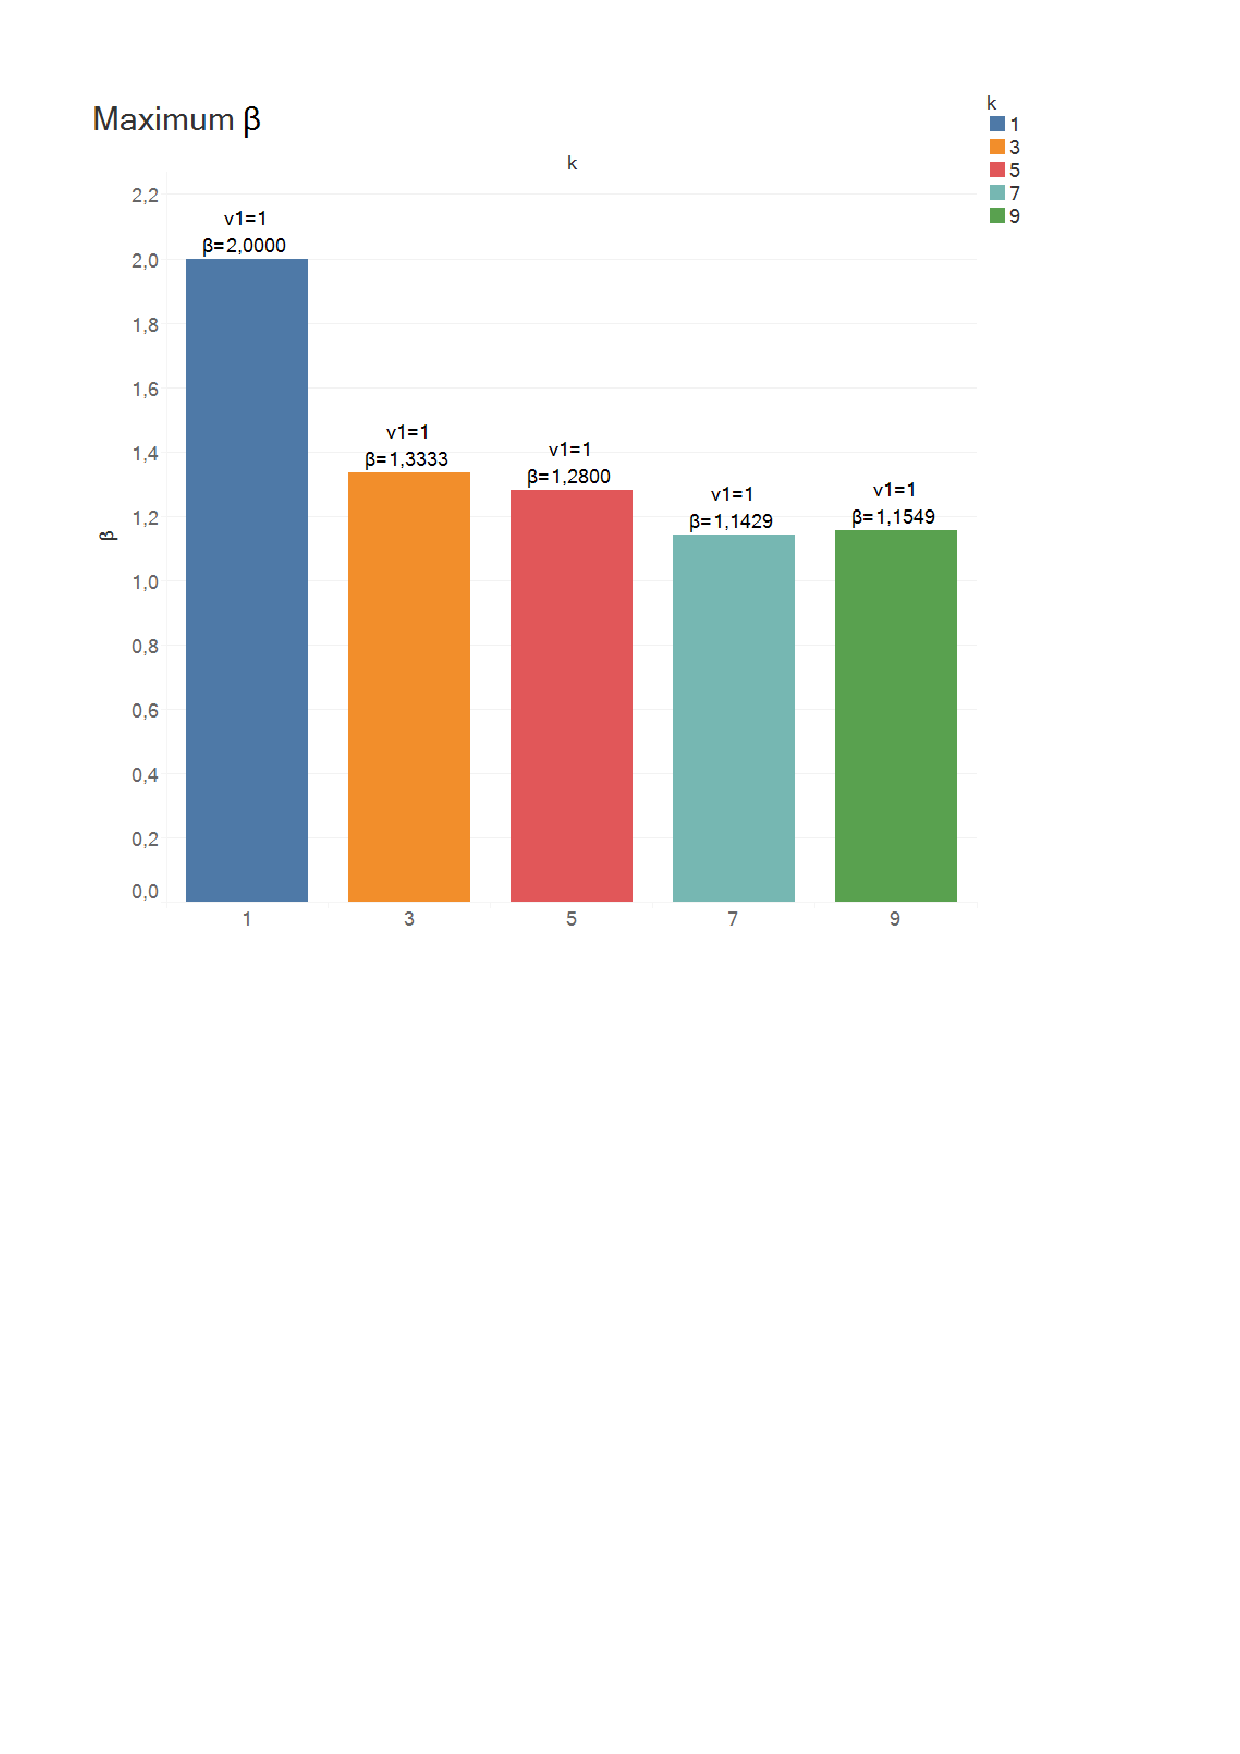
\includegraphics[trim=40 45 60 40, clip, width=1.0\textwidth]{figures/beta_dashboard.pdf}
\caption{Maximum $\beta$ for different $k$}
\label{fig:1}
\end{center}
\end{figure}

As we can see from figure~\ref{fig:1}, the maximum for $k=1$ equals $2$. The limit for the other $k$ is beneath. For example, the maximum for $k=3$ equals $1.\overline{3}=\frac{4}{3}$. The diagram reveals that the maximum $\beta$ for every $k$ is reached for the starting number $v_1=1$. A proof for this finding will be provided in a future article. In the next section we will discuss the implications of theorem~\ref{eq:boundary_beta} on the occurrence of cycles.

\vspace{1em}\noindent
\subsection{Analysing \boldmath$\bar\alpha$}
\par\noindent
How many divisions by two can lead to a cycle within a Collatz sequence? We can derive an equation for this number, subsequently called $\bar\alpha$, on the basis of formula~\ref{eq:reachability_k} and theorem \ref{eq:boundary_beta}. Therefore, we examine the case in which equation~\ref{eq:reachability_k} leads to a cycle by setting $v_{n+1}=v_1$:
\begin{equation}
\label{eq:cycle_alpha}
\def\arraystretch{1.2}\begin{array}{l}
	v_1=k^n\cdot v_1\cdot\beta\cdot2^{-\bar\alpha}\\
	2^{\bar\alpha}=k^n\cdot\beta\\
	\bar\alpha=n\cdot\log_2k+\log_2\beta\\
	\bar\alpha=\lfloor n\cdot\log_2k\rfloor+1
\end{array}
\end{equation}

The last transformation above is applied, since $\bar\alpha$ is a whole number.\footnote{Accordingly, the sum of the mantissas of $n\cdot\log_2k+\log_2\beta$ must be one.} Now that it is clear that $1<\beta\le2$, we truncate the fractional part of $(n\cdot \log_2k)$ and add one to the result. In a Collatz sequence a cycle can only occur if the number of divisions by two equals $\bar\alpha$. Conversely, this does not imply that reaching $\bar\alpha$ inevitably leads to a cycle. The following example demonstrates this. Let us consider the case where $k=3$, $v_1=83$ and $n=3$. Here, theorem~\ref{eq:cycle_alpha} and formula~\ref{eq:reachability_k} yield the following result:
\[
\def\arraystretch{1.2}\begin{array}{c}
\bar\alpha=5=\lfloor3\cdot\log_23\rfloor+1\\
71=3^3\cdot83\cdot\left(1+\frac{1}{3\cdot83}\right)\cdot\left(1+\frac{1}{3\cdot125}\right)\cdot\left(1+\frac{1}{3\cdot47}\right)\cdot2^{-5}
\end{array}
\]

\par
Before we continue, we will empirically validate theorem~\ref{eq:cycle_alpha}. Our tool is a linear search performed by a Python script. For details on the program see section "\nameref{appx:cycle_finder}" in the appendix. With the script we searched and evaluated cycles in Collatz sequences for the odd starting numbers $v_1\in\{1,3,5,\ldots,9999\}$ and $k\in\{1,3,5,\ldots,999\}$. In order to restrict the runtime of the program we limited the length of the investigated cycles to $n=100$. The results of our empirical validation are shown in the following table.

\begin{table}[H]
	\centering
	\setlength{\tabcolsep}{1,2em}
	\begin{tabular}{|L|R|R|R|C|}
		\hline
		\thead{\boldsymbol{k}} &
		\thead{\boldsymbol{v_1\mathrel{{.}\,{.}}v_n}} &
		\thead{\boldsymbol{n}} &
		\thead{\boldsymbol{\alpha}} &
		\thead{\boldsymbol{\bar\alpha}}\\
		\hline
		1 &
		(1) &
		1 &
		1 &
		1\\
		\hline
		3 &
		(1) &
		1 &
		2 &
		2\\
		\hline
		5 &
		(1,3) &
		2 &
		5 &
		5\\
		\hline
		5 &
		(13,33,83) &
		3 &
		7 &
		7 \\
		\hline
		5 &
		(27,17,43) &
		3 &
		7 &
		7 \\
		\hline
		7 &
		(1) &
		1 &
		3 &
		3\\
		\hline
		15 &
		(1) &
		1 &
		4 &
		4\\
		\hline
		31 &
		(1) &
		1 &
		5 &
		5\\
		\hline
		63 &
		(1) &
		1 &
		6 &
		6\\
		\hline
		127 &
		(1) &
		1 &
		7 &
		7\\
		\hline
		181 &
		(27,611) &
		2 &
		15 &
		15\\
		\hline
		181 &
		(35,99) &
		2 &
		15 &
		15\\
		\hline
		255 &
		(1) &
		1 &
		8 &
		8\\
		\hline
		511 &
		(1) &
		1 &
		9 &
		9\\
		\hline
	\end{tabular}
	\caption{Cycles in Collatz sequences}
	\label{table:known_cycles}
\end{table}

As one can see in table~\ref{table:known_cycles}, we found several cycles for our generalised form of the Collatz problem. All of which comply with theorem~\ref{eq:cycle_alpha}.\footnote{Source: Own empirical analysis, see appendix "\nameref{appx:cycle_finder}" for details.}

\vspace{1em}\noindent
\subsection{Binary Growth}
\par\noindent
As we have emphasised at several points in this paper, theorem~\ref{eq:max_alpha} builds on the binary length of the starting value $len(v_1)$. Furthermore, it accounts for the maximum binary growth, henceforth denoted with $\hat\Lambda$. We define binary growth as the total number of digits by which the binary length of $v_1$ increases in a sequence.\footnote{This means that $\hat\Lambda$ does not account for the divisions by two that reduce the binary length of $v_1$.} In order to reach the final result $v_{n+1}=len(v_{n+1})=1$, we have to substract $\hat\alpha$ from the sum of the binary length of $v_1$ and the binary growth:
\begin{equation}
\label{eq:binary_growth}
\def\arraystretch{1.2}\begin{array}{l}
1=len(v_1)+\hat\Lambda-\hat\alpha\\
\hat\Lambda=\hat\alpha+1-len(v_1)\\
\hat\Lambda=\lfloor n\cdot\log_2k+\log_2v_1\rfloor+1+1-\lfloor\log_2v_1\rfloor-1\\
\hat\Lambda=\lfloor n\cdot\log_2k+\log_2v_1\rfloor+1-\lfloor\log_2v_1\rfloor\\
\lfloor n\cdot\log_2k\rfloor+1\le\hat\Lambda\le\lfloor n\cdot\log_2k\rfloor+2
\end{array}
\end{equation}

In the final step the above equation is condensed by subtracting the starting value $v_1$. As a result, we obtain a range for $\hat\Lambda$. The reason is a possible overflow which can be instigated by the expression $n\cdot\log_2k+\log_2v_1$. Let us examine two examples to illustrate this. Starting with the case $k=3$, $v_1=13$ and $n=2$ we find that the result is equal to the lower limit of $\hat\Lambda$:

\[
\hat\Lambda=\lfloor2\cdot\log_23+\log_213\rfloor+1-\lfloor\log_213\rfloor=\lfloor2\cdot\log_23\rfloor+1=4
\]

\par\medskip
Setting $v_1=7$, $k=3$ and $n=5$ leads to the upper limit of the variable:
\[
\hat\Lambda=\lfloor5\cdot\log_23+\log_27\rfloor+1-\lfloor\log_27\rfloor=\lfloor5\cdot\log_23\rfloor+2=9
\]

The parameter $\hat\Lambda$ represents the maximum binary growth of a Collatz sequence. In other words, the binary growth of a sequence cannot exceed $\hat\Lambda$, even if we would not perform any divisions by two. Examining formula~\ref{eq:binary_growth}, it is not surprising that we find the following relation to theorem~\ref{eq:cycle_alpha}:
\[
\bar\alpha=\lfloor n\cdot\log_2k\rfloor+1\le\hat\Lambda
\]
As we know, a cycle occurs in a Collatz sequence when the condition $v_1=v_{n+1}$ is fulfilled. The binary length of the starting number $v_1$, must therefore grow exactly as much as it is reduced by the divisions by two. Thus, for a cycle to occur, the number of divisions by two has to be equal to the binary growth.

\par\medskip
One might argue that this reasoning is erroneous since a sequence does not necessarily reach the maximum binary growth. We build on formula~\ref{eq:reachability_k} to show that our arguments are valid. By setting $v_{n+1}=v_1$ we examine the case where the growth of the binary length of a sequence is neutralised by the divisions by two:
\[
\begin{array}{l}
v_1=k^n\cdot v_1\cdot\beta\cdot2^{-\alpha}\\
2^{\alpha}=k^n\cdot\beta\\
\alpha=n\cdot\log_2k+log_2\beta
\end{array}
\]

Knowing that $1<\beta\le2$, we derive the following limits for the binary growth of a cycle, subsequently called $\bar\Lambda$:
\[
n\cdot\log_2k<\bar\Lambda\le\lfloor n\cdot\log_2k\rfloor+1
\]

The binary growth of every Collatz sequence that leads to a cycle must lie within these boundaries. Due to the fact that $\bar\alpha$ is a whole number, it is obvious that it must equal the maximum on the right side of the expression. For all other cases a cycle is impossible.

\section{Summary}
In our paper we have shed light on a central aspect of the Collatz conjecture: the divisions by two. We analysed the problem in its original form $3v+1$ as well as in the generalised variant $kv+1$. Based on mathematical reasoning and empirical studies we derived and proved theorems on the occurrence of cycles and the termination of sequences. Our reasoning primarily builds on the binary representation of Collatz numbers and the underlying operations. Theorem~\ref{eq:cycle_alpha} determines the number of divisions by two that can lead to a cycle. The theorem is based on the simple truth that a cycle can only occur if the binary growth of a sequence is exactly neutralised by the divisions by two. Theorem~\ref{eq:max_alpha} determines the maximum number of divisions by two that can be performed in a sequence. If one could show that every starting number finally leads to this maximum, the Collatz problem would be solved. We are convinced that a profound study of the binary mechanics of Collatz sequences will lead to this proof.\\

\par\bigskip\noindent
{\titleformat{Appendix}}
\section{Data Set}
\label{appx:data_set}
This empirical data set was used to derive and validate theorems~\ref{eq:boundary_alpha_i}, \ref{eq:max_alpha} and \ref{eq:boundary_beta}. The sample was generated with a Python script and comprises information about sequences for the odd starting numbers $v_1\in\{1,3,5,\ldots,3999\}$ and $k\in\{1,3,5,7,9\}$.\footnote{\url{https://github.com/c4ristian/collatz/blob/v1.3/run_alpha_export.py}} Since we do not know that all generated sequences halt, we limited the number of iterations per sequence to $n=100$. In total, the sample contains 651,159 Collatz numbers, which are not necessarily distinct. This is due to the fact that different starting numbers can lead to the same subsequent values. For example, both starting values, $v_1=13$ and $v_1=53$, result in the number five.

\section{Cycle Finder}
\label{appx:cycle_finder}
This Python script was used to validate theorem~\ref{eq:cycle_alpha}.\footnote{\url{https://github.com/c4ristian/collatz/blob/v1.3/run_cycle_finder.py}} The program performs a linear search for the odd starting numbers $v_1\in\{1,3,5,\ldots,9999\}$ and $k\in\{1,3,5,\ldots,999\}$. To restrict the runtime of the script, we limited the length of the investigated cycles to $n=100$. Furthermore, the results are not persisted. In order to reproduce our findings, the program must be executed again.

\section{Scientific Approach}
\label{appx:scientific_approach}
The contents published in this paper have been achieved with an interdisciplinary approach. Not surprising, we applied classic mathematical theory and reasoning. Since we are convinced that the Collatz problem cannot be solved with traditional maths alone, we additionally used techniques of data science. We combined the two fields in different ways. On one hand, we analysed sequences and related features empirically, in order to derive new formulas and theorems. On the other hand, we used data science to validate our proofs. As suggested by Karl Popper, we tried to falsify them with counterexamples. In the course of our work, we have learned that the combination of the two fields leads to a very efficient working mode. This might be the topic of another paper.

\section{Alternative Verification of \boldmath{$\hat\alpha$}}
\label{appx:alternative_verification_max_alpha}
We can alternatively verify theorem~\ref{eq:max_alpha} for $k=3$ with the following equation. Formula~\ref{eq:engel} builds on the so-called Engel expansion and calculates the odd number $v_{n+1}$ for a Collatz sequence in which we divide by two only once per iteration:\footnote{See Laarhoven, 2009 \cite[p.~11]{Ref_Laarhoven_2009}}

\begin{equation}
\label{eq:engel}
v_{n+1}=\frac{3^n*(v_1+1)-2^n}{2^n}
\end{equation}

\par\noindent
The above term represents the (hypothetical) case in which a sequence rises to its maximum for a specific starting value $v_1$. For the Collatz conjecture this scenario can be considered as worst-case, as it never ends with one due to its steady increase. Let us consider the example $v_1=7$ and $n=1$. Applying equation~\ref{eq:engel} yields:
\[
v_{1+1}=\frac{3^1*(7+1)-2^1}{2^1}=11
\]

\par\noindent
Setting $v_1=31$ and $n=3$ leads to:
\[
v_{3+1}=\frac{3^3*(7+1)-2^3}{2^3}=107
\]

\par\noindent
We use formula~\ref{eq:engel} to verify theorem~\ref{eq:max_alpha} by proving that dividing $\hat\alpha$ times by two will lead to a result $v_{n+2}<2$ for every worst-case sequence. For this purpose, we extend formula~\ref{eq:engel} by an additional step and divide by $\hat\alpha-n$ in the final iteration:
\[
v_{n+2}=\left[ \left(\frac{3^n*(v_1+1)-2^n}{2^n}\right)*3+1\right]*2^{-(\hat\alpha-n)}
\]

\par\noindent
We assume that the sequence leads to a result $v_{n+2}<2$ and thus verify theorem~\ref{eq:max_alpha}:\footnote{The case is hypothetical. Not every worst-case sequence actually ends with $v_{n+2}=1$. We consequently have to define the condition $v_{n+2}<2$ in order to cover all possible sequences.}
\begin{equation}
\def\arraystretch{1.2}\begin{array}{l}
2>\left[ \left(\frac{3^n*(v_1+1)-2^n}{2^n}\right)*3+1\right]*2^{-(\hat\alpha-n)}\\
2^{\hat\alpha-n+1}>\left[ \left(\frac{3^n*(v_1+1)-2^n}{2^n}\right)*3+1\right]\\
2^{\hat\alpha-n+1}-1>\frac{3^{n+1}*(v_1+1)-3*2^n}{2^n}\\
2^{\hat\alpha+1}-2^n>3^{n+1}*(v_1+1)-3*2^n\\
2^{\hat\alpha+1}-2^n+3*2^n>3^{n+1}*(v_1+1)\\
2^{\hat\alpha+1}+2^{n+1}>3^{n+1}*(v_1+1)\\
2^{\lfloor n\cdot\log_23+\log_2v_1\rfloor+2}+2^{n+1}>3^{n+1}*(v_1+1)\\
\end{array}
\end{equation}

\par\noindent
When resolving $\hat\alpha$ in the last transformation above we have to use the factor $n+1$, since we have extended our worst-case sequence by an additional iteration. Even though it is not obvious at the first glance, the above condition is true for any given $n$ and $v_1$. This verifies theorem~\ref{eq:max_alpha} for $k=3$, at least for all worst-case sequences. As the attentive reader will realise the verification is valid for all $k$. We will elaborate on this topic more deeply in a future article focusing on the role of the Engel expansion in Collatz sequences.

\vfill

\section{Glossary of Notations}
\label{appx:glossary_of_notations}
\vspace{-1em}
\begin{table}[H]
	\centering
	\setlength{\tabcolsep}{1,2em}\setlength\extrarowheight{3pt}
	\begin{tabular}{|l|p{13.5cm}|}
		\hline
		\thead{\textbf{Notation}} &
		\thead{\textbf{Description}}\\
		\hline
		$v_1$ &
		First odd number of a Collatz sequence, also referred to as starting value\\
		\hline
		$v_i$ &
		Odd number that is the result of a particular iteration. In the first iteration this is the starting value $v_1$\\
		\hline
		$k$ &
		Factor that is multiplied with odd numbers; equals three for the original Collatz conjecture\\
		\hline
		$n$ &
		Count of odd numbers in a sequence, also referred to as the sequence's length\\
		\hline
		$\beta_i$ &
		Symbolises the term $\left(1+\frac{1}{k\cdot v_i}\right)$\\
		\hline
		$\beta$ &
		Product of all $\beta_i$\\
		\hline
		$\alpha_i$ &
		Represents the number of divisions by two that are performed in a specific iteration\\
		\hline
		$\alpha$ &
		Number of divisions by two that leads from the starting value $v_1$ to the result $v_{n+1}$\\
		\hline
		$\hat\alpha_i$ &
		Maximum possible number of divisions by two in a specific iteration\\
		\hline
		$\hat\alpha$ &
		Maximum possible number of divisions by two in a Collatz sequence\\
		\hline
		$\bar\alpha$ &
		Number of divisions by two that is required for a cycle\\
		\hline
		$\hat\Lambda$ &.md
		Maximum binary growth of a Collatz sequence\\
		\hline
		$\bar\Lambda$ &
		Binary growth that is required for a cycle\\
		\hline
	\end{tabular}
\end{table}


\vspace{1em}
\begin{thebibliography}{99}

\bibitem{Ref_Lagarias_2010}
J. C. Lagarias: The Ultimate Challenge: The 3x+1 Problem. American Mathematical Society, 2010, ISBN 978-0821849408

\bibitem{Ref_Sultanow_Koch_Cox_2020}
E. Sultanow, C. Koch and S. Cox: Collatz Sequences in the Light of Graph Theory (Fourth Version). University of Potsdam, 2020, DOI https://doi.org/10.25932/publishup-44325

\bibitem{Ref_Sedgewick_Wayne_2011}
R. Sedgewick and K. Wayne: Algorithms (Fourth Edition). Addison-Wesley Professional, 2011, ISBN 978-0321573513

\bibitem{Ref_Laarhoven_2009}
T.M.M. Laarhoven: The 3n + 1 conjecture. Eindhoven University of Technology, July 2009.

\end{thebibliography}


\end{document}